% fig_3_1_augmentation_taxonomy.tex
% Hierarchical tree of data augmentation methods for NLP
% Compile: pdflatex fig_3_1_augmentation_taxonomy.tex
\documentclass[tikz,border=5pt]{standalone}

\usepackage[T1]{fontenc}
\usepackage[utf8]{inputenc}
\usepackage{amsmath,amssymb}
\usepackage{tikz}
\usetikzlibrary{arrows.meta, positioning, shapes.geometric, calc, trees, decorations.pathreplacing}

% ── Color palette ──────────────────────────────────────────────────
\definecolor{rootColor}{HTML}{263238}
\definecolor{branchColor}{HTML}{37474F}
\definecolor{baselineBlue}{HTML}{1565C0}
\definecolor{baselineBlueFill}{HTML}{E3F2FD}
\definecolor{referencedGray}{HTML}{757575}
\definecolor{referencedGrayFill}{HTML}{F5F5F5}
\definecolor{proposedGold}{HTML}{F9A825}
\definecolor{proposedGoldFill}{HTML}{FFF8E1}
\definecolor{hybridPurple}{HTML}{7B1FA2}
\definecolor{hybridPurpleFill}{HTML}{F3E5F5}
\definecolor{arrowGray}{HTML}{546E7A}
\definecolor{starGold}{HTML}{FFD600}

\begin{document}
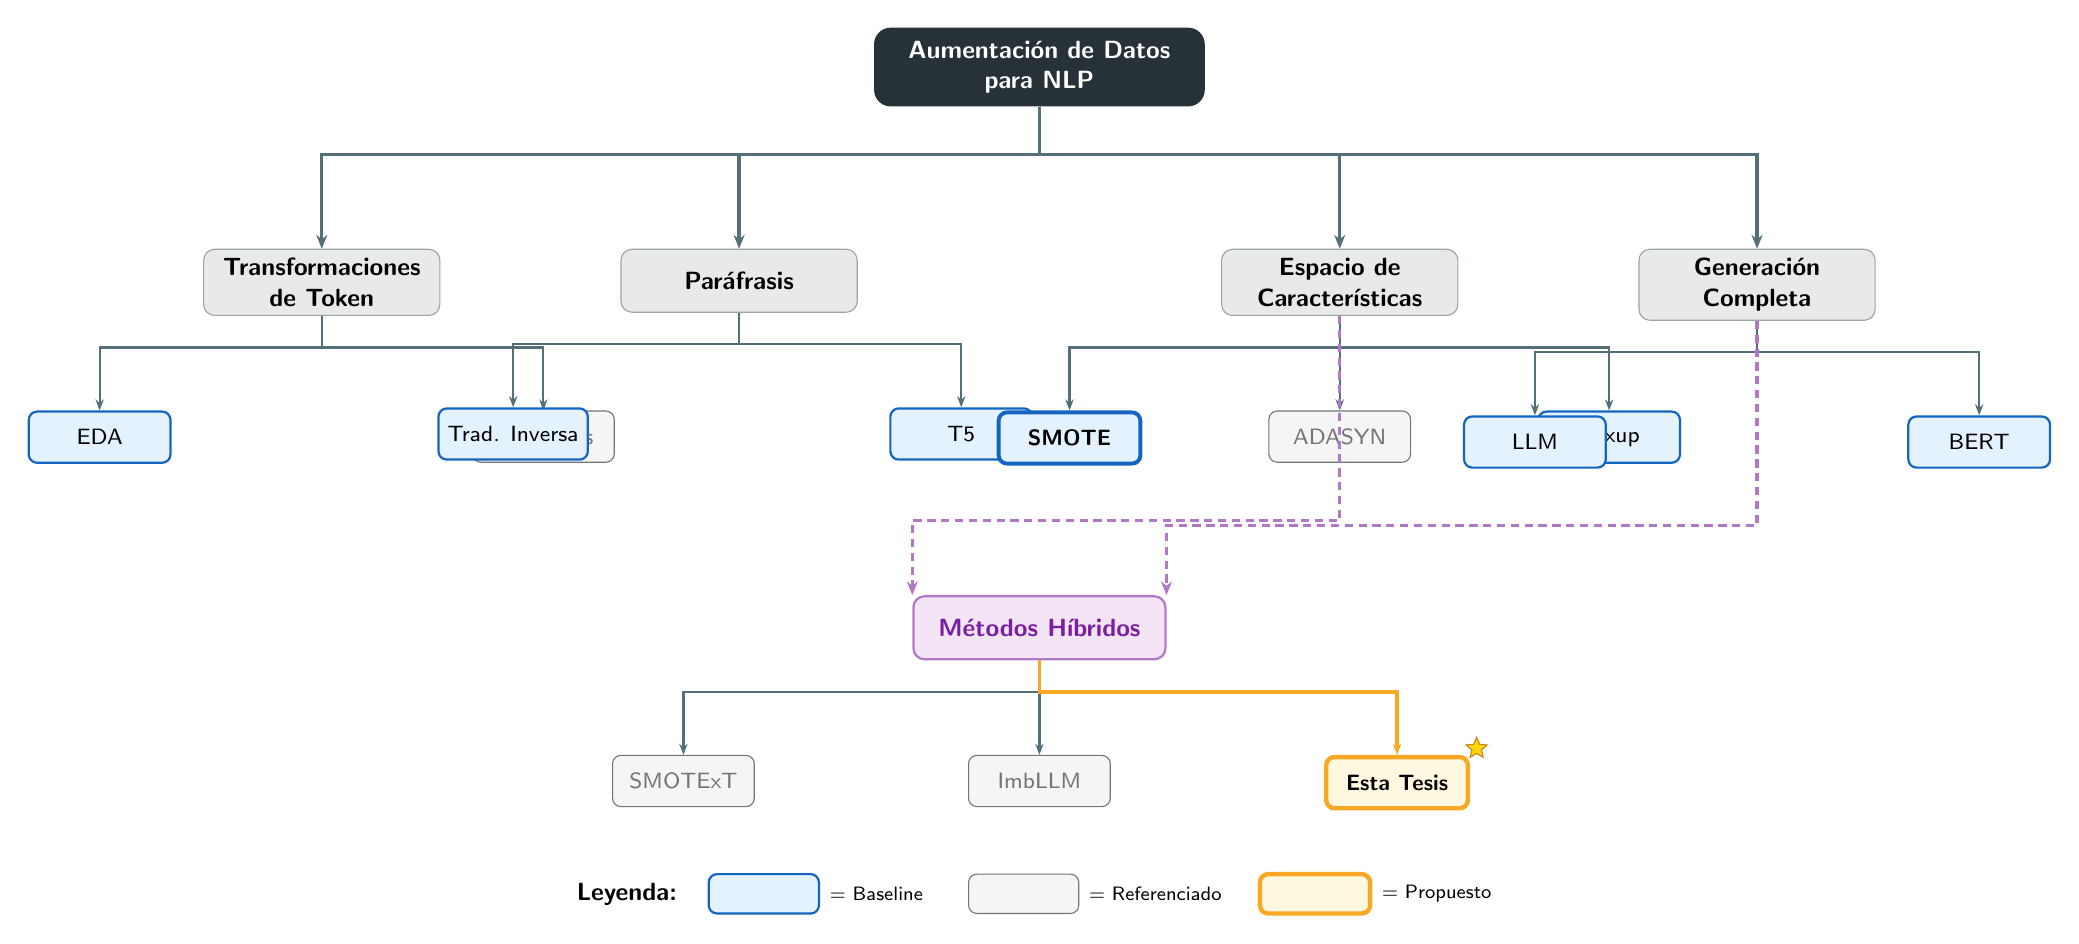
\begin{tikzpicture}[
    % ── shared styles ───────────────────────────────────────────────
    rootnode/.style={
        rectangle, rounded corners=6pt,
        fill=rootColor, text=white,
        font=\sffamily\bfseries\small,
        minimum height=1.0cm, minimum width=4.2cm,
        align=center,
    },
    branch/.style={
        rectangle, rounded corners=4pt,
        fill=branchColor!12, draw=branchColor!50,
        font=\sffamily\small\bfseries,
        minimum height=0.8cm, minimum width=3.0cm,
        align=center,
    },
    baseline/.style={
        rectangle, rounded corners=3pt,
        fill=baselineBlueFill, draw=baselineBlue, thick,
        font=\sffamily\footnotesize,
        minimum height=0.65cm, minimum width=1.8cm,
        align=center,
    },
    baseline bold/.style={
        baseline, font=\sffamily\footnotesize\bfseries,
        line width=1.4pt,
    },
    referenced/.style={
        rectangle, rounded corners=3pt,
        fill=referencedGrayFill, draw=referencedGray,
        font=\sffamily\footnotesize, text=referencedGray,
        minimum height=0.65cm, minimum width=1.8cm,
        align=center,
    },
    proposed/.style={
        rectangle, rounded corners=3pt,
        fill=proposedGoldFill, draw=proposedGold, line width=1.6pt,
        font=\sffamily\footnotesize\bfseries,
        minimum height=0.65cm, minimum width=1.8cm,
        align=center,
    },
    hybrid branch/.style={
        rectangle, rounded corners=4pt,
        fill=hybridPurpleFill, draw=hybridPurple!60, thick,
        font=\sffamily\small\bfseries, text=hybridPurple,
        minimum height=0.8cm, minimum width=3.2cm,
        align=center,
    },
    conn/.style={
        -{Stealth[length=4pt,width=3pt]},
        arrowGray, line width=0.8pt,
    },
    conn thick/.style={
        -{Stealth[length=5pt,width=4pt]},
        arrowGray, line width=1.2pt,
    },
]

% =============================================================
%  ROOT
% =============================================================
\node[rootnode] (root) at (0,0) {Aumentaci\'{o}n de Datos\\para NLP};

% =============================================================
%  BRANCH 1: Transformaciones de Token
% =============================================================
\node[branch, below left=1.8cm and 5.5cm of root] (b1) {Transformaciones\\de Token};
\draw[conn thick] (root.south) -- ++(0,-0.6) -| (b1.north);

% Leaves
\node[baseline, below left=1.2cm and 0.4cm of b1] (eda) {EDA};
\node[referenced, below right=1.2cm and 0.4cm of b1] (sinon) {Sin\'{o}nimos};
\draw[conn] (b1.south) -- ++(0,-0.4) -| (eda.north);
\draw[conn] (b1.south) -- ++(0,-0.4) -| (sinon.north);

% =============================================================
%  BRANCH 2: Parafrasis
% =============================================================
\node[branch, below left=1.8cm and 0.2cm of root] (b2) {Par\'{a}frasis};
\draw[conn thick] (root.south) -- ++(0,-0.6) -| (b2.north);

% Leaves
\node[baseline, below left=1.2cm and 0.4cm of b2] (trad) {Trad. Inversa};
\node[baseline, below right=1.2cm and 0.4cm of b2] (t5) {T5};
\draw[conn] (b2.south) -- ++(0,-0.4) -| (trad.north);
\draw[conn] (b2.south) -- ++(0,-0.4) -| (t5.north);

% =============================================================
%  BRANCH 3: Espacio de Caracteristicas
% =============================================================
\node[branch, below right=1.8cm and 0.2cm of root] (b3) {Espacio de\\Caracter\'{i}sticas};
\draw[conn thick] (root.south) -- ++(0,-0.6) -| (b3.north);

% Leaves
\node[baseline bold, below left=1.2cm and 1.0cm of b3] (smote) {SMOTE};
\node[referenced, below=1.2cm of b3] (adasyn) {ADASYN};
\node[baseline, below right=1.2cm and 1.0cm of b3] (mixup) {Mixup};
\draw[conn] (b3.south) -- ++(0,-0.4) -| (smote.north);
\draw[conn] (b3.south) -- ++(0,-0.4) -| (adasyn.north);
\draw[conn] (b3.south) -- ++(0,-0.4) -| (mixup.north);

% =============================================================
%  BRANCH 4: Generacion Completa
% =============================================================
\node[branch, below right=1.8cm and 5.5cm of root] (b4) {Generaci\'{o}n\\Completa};
\draw[conn thick] (root.south) -- ++(0,-0.6) -| (b4.north);

% Leaves
\node[baseline, below left=1.2cm and 0.4cm of b4] (llm) {LLM};
\node[baseline, below right=1.2cm and 0.4cm of b4] (bert) {BERT};
\draw[conn] (b4.south) -- ++(0,-0.4) -| (llm.north);
\draw[conn] (b4.south) -- ++(0,-0.4) -| (bert.north);

% =============================================================
%  HYBRID BRANCH (from branches 3+4)
% =============================================================
\node[hybrid branch, below=6.2cm of root] (hybrid) {M\'{e}todos H\'{i}bridos};

% Connection lines from B3 and B4 into hybrid
\draw[conn thick, hybridPurple!60, densely dashed]
  (b3.south) -- ++(0,-2.6) -| (hybrid.north west);
\draw[conn thick, hybridPurple!60, densely dashed]
  (b4.south) -- ++(0,-2.6) -| (hybrid.north east);

% Hybrid leaves
\node[referenced, below left=1.2cm and 2.0cm of hybrid] (smotex) {SMOTExT};
\node[referenced, below=1.2cm of hybrid] (imbllm) {ImbLLM};
\node[proposed, below right=1.2cm and 2.0cm of hybrid] (thesis) {Esta Tesis};

\draw[conn] (hybrid.south) -- ++(0,-0.4) -| (smotex.north);
\draw[conn] (hybrid.south) -- ++(0,-0.4) -| (imbllm.north);
\draw[conn, proposedGold, line width=1.2pt] (hybrid.south) -- ++(0,-0.4) -| (thesis.north);

% Star on proposed node
\node[star, star points=5, star point ratio=2.2,
      fill=starGold, draw=proposedGold!80!black,
      inner sep=0pt, minimum size=8pt,
      anchor=south west] at (thesis.north east) {};

% =============================================================
%  LEGEND
% =============================================================
\begin{scope}[shift={(-6.0, -10.5)}]
  \node[font=\sffamily\small\bfseries, anchor=west] at (0, 0) {Leyenda:};

  \node[baseline, minimum width=1.4cm, minimum height=0.5cm] (legB) at (2.5, 0) {};
  \node[font=\sffamily\scriptsize, anchor=west] at (legB.east) { = Baseline};

  \node[referenced, minimum width=1.4cm, minimum height=0.5cm] (legR) at (5.8, 0) {};
  \node[font=\sffamily\scriptsize, anchor=west] at (legR.east) { = Referenciado};

  \node[proposed, minimum width=1.4cm, minimum height=0.5cm] (legP) at (9.5, 0) {};
  \node[font=\sffamily\scriptsize, anchor=west] at (legP.east) { = Propuesto};
\end{scope}

\end{tikzpicture}
\end{document}
